% !TEX root = ../../I4PRJ, Grp3 - Dokumentation.tex
\section{Web}
I dette afsnit beskrives designet af Web-applikationen. Designet benytter ASP.NET MVC framework. Controllerklasserne er lavet således, at de implementerer hvert view-interface i præsentationslaget. Broen mellem ASP.NET MVC og den overordnede MVP arkitektur sker altså ved implementering af førnævnte interfaces.
\begin{figure}
	\centering
	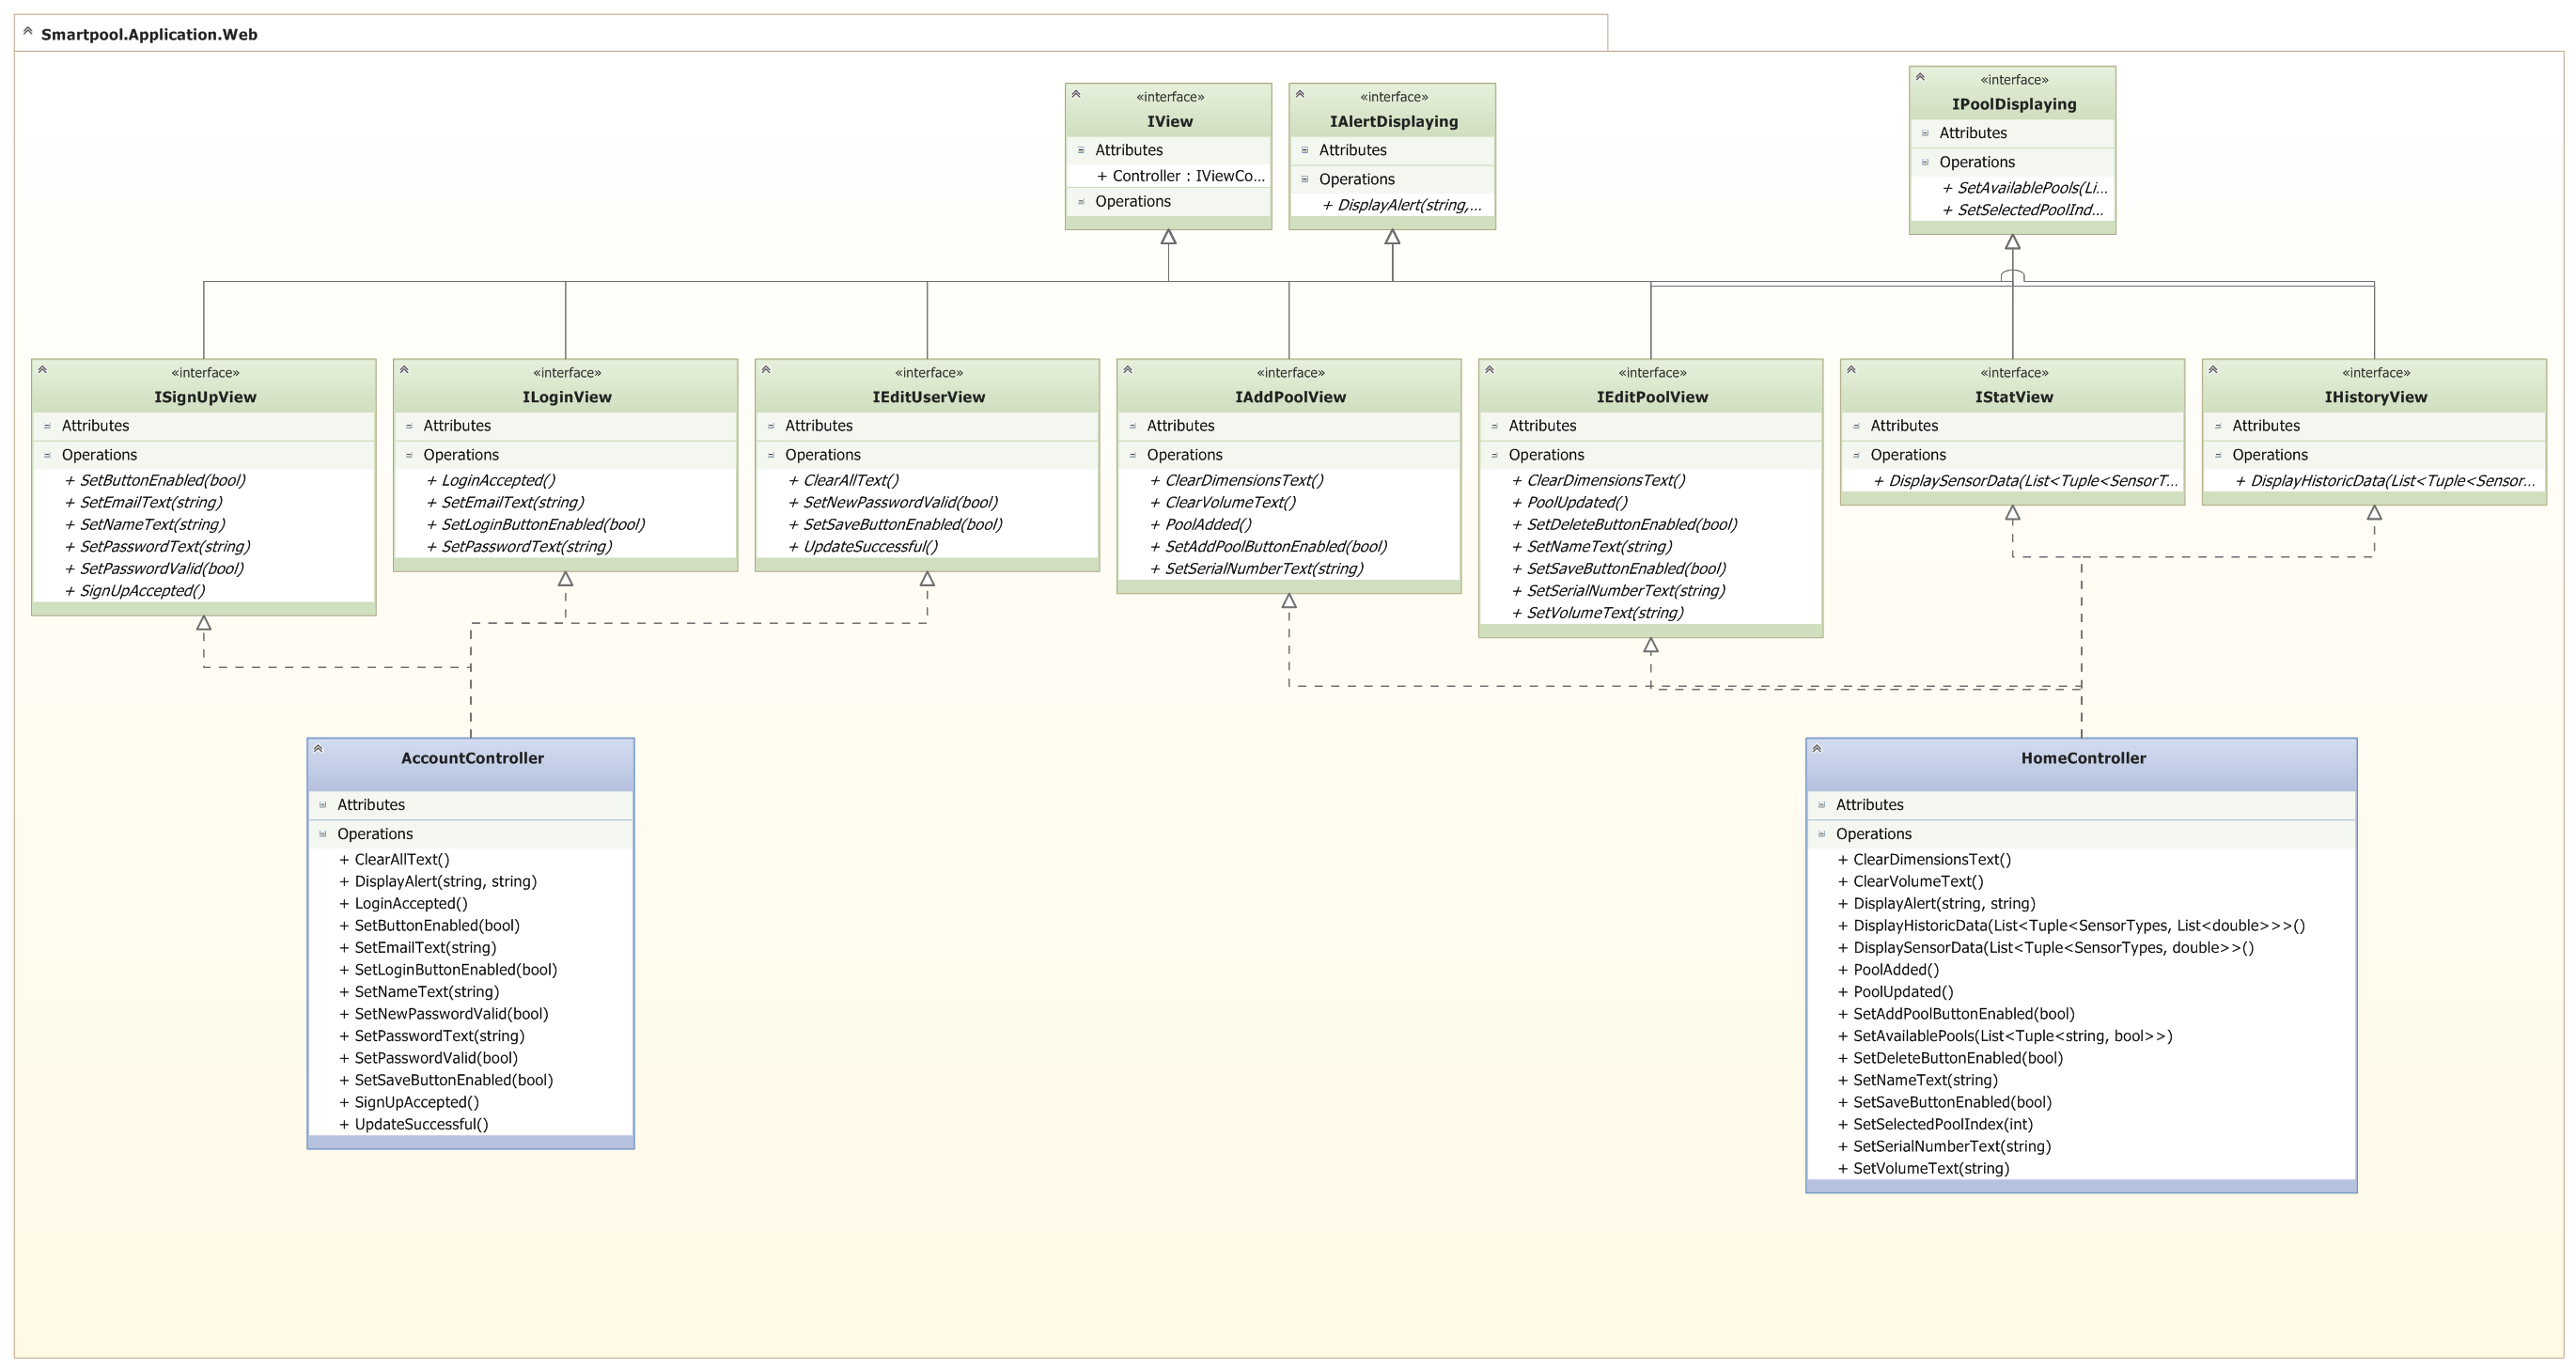
\includegraphics[width=0.9\linewidth]{figs/design/application_web}
	\caption{Web applikations design}
	\label{fig:web_class}
\end{figure}

